\draft Electronic properties under magnetic field.

\begin{parts}
	\part
	\begin{figure}[H]
		\centering
			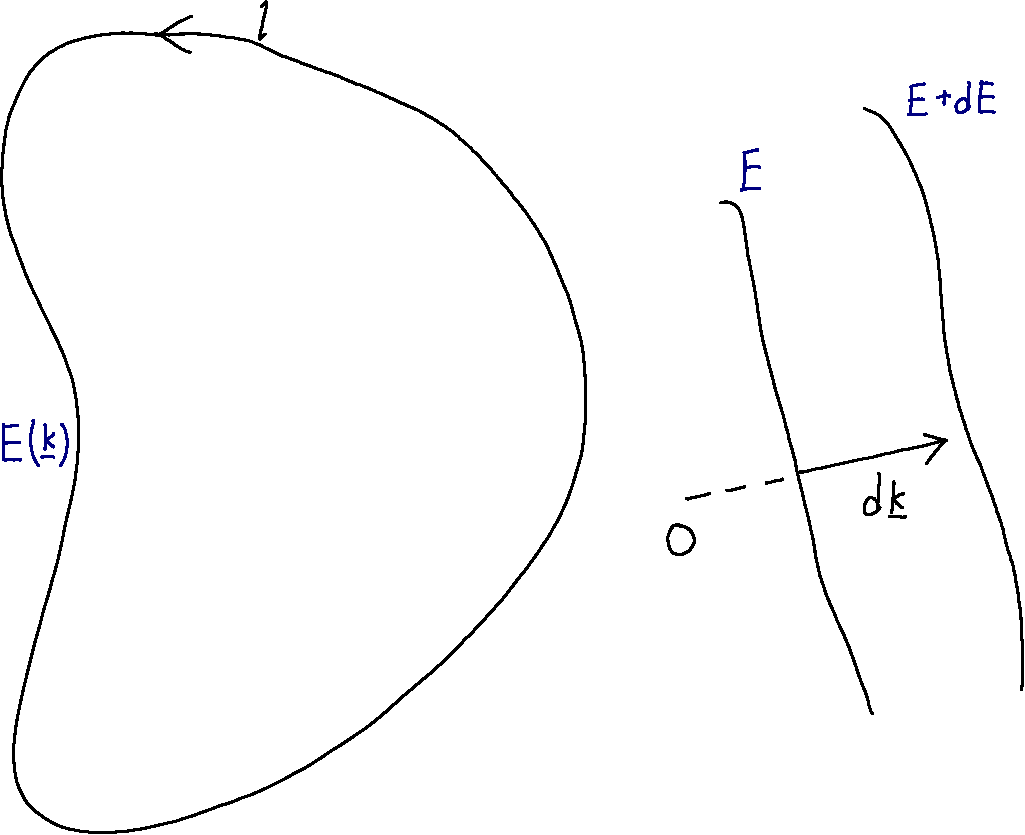
\includegraphics[width=.7\linewidth]{q3-dE}
	\end{figure}
	In 2D, the d.o.s. may be written as $g(k) \inftsml{k} = \inftsml{A}$ where $\inftsml{A}$ is an areal loop element of equal energy.
	
	Also we have dispersion $E(\mathbf{k}) \Rightarrow \mathbf{\nabla}E = \nabla E \hat{\mathbf{n}}$ where $\hat{\mathbf{n}}$ is the normal to the isoenergy line $l$.
	
	\todo We know that:
	\begin{align*}
		\inftsml{E} &= \mathbf{\nabla}E \cdot \inftsml{\mathbf{k}} \\
		&= \nabla E \inftsml{k} \rbracket{\hat{\mathbf{n}} \cdot \hat{\mathbf{n}}} \\
		\Rightarrow \inftsml{k} &= \frac{\inftsml{E}}{\nabla E}
	\end{align*}
	
	$\inftsml{A}$ is then:
	\begin{align*}
		\inftsml{A} &= \oint \inftsml{l} \cdot \inftsml{k} \\
		&= \oint \frac{\inftsml{l}}{\nabla E} \inftsml{E} \\
		\Rightarrow g(E) &= \oint \frac{\inftsml{l}}{\nabla E}
	\end{align*}
	Prefactor $1/(2\pi)^n$ from continuum approx.
	
	In 1D, we have $\inftsml{E} / \nabla E = g(E) \inftsml{E}$ instead.
	
	\part
	\begin{align*}
		\mathcal{H} &= \frac{\hat{p_x^2}}{2m_1} + \frac{\rbracket{\hat{p_y} + eB_z x}^2}{2m_2} \\
		\Rightarrow \mathcal{H} &= \frac{\hat{p_x^2}}{2m_1} + \frac{\rbracket{\hbar k_y + eB_z x}^2}{2m_2}
	\end{align*}
	since $\sbracket{\mathcal{H}, \hat{p_y}} = 0$ allows us to write the eigenvalue in place.
	
	Let $-\hbar k_y / eB = x_0$:
	\begin{align*}
		\mathcal{H} &= \frac{\hat{p_x^2}}{2m_1} + \frac{\rbracket{eB_z}^2}{2m_2} \rbracket{x - x_0}^2 \\
		&= \frac{1}{2m_1} \hat{p_x^2} + \frac{1}{2} m_1 \omega^2 \rbracket{x - x_0}^2
	\end{align*}
	
	Note that the form of Hamiltonian is that of a harmonic oscillator, thus we have $\omega = eB / \sqrt{m_1 m_2}$ and energy eigenvalue $E_l = (l + 1/2)\hbar\omega$ with $l \in \mathcal{Z}$.
	
	Gauge changing will introduce additional terms, and thus constant to the energy eigenvalue, however it has no physical meaning as only energy difference is observable.
	
	\part Density of states in a real system: (broadening due to scattering and imperfections in 2D geometry):
	\begin{figure}[H]
		\centering
		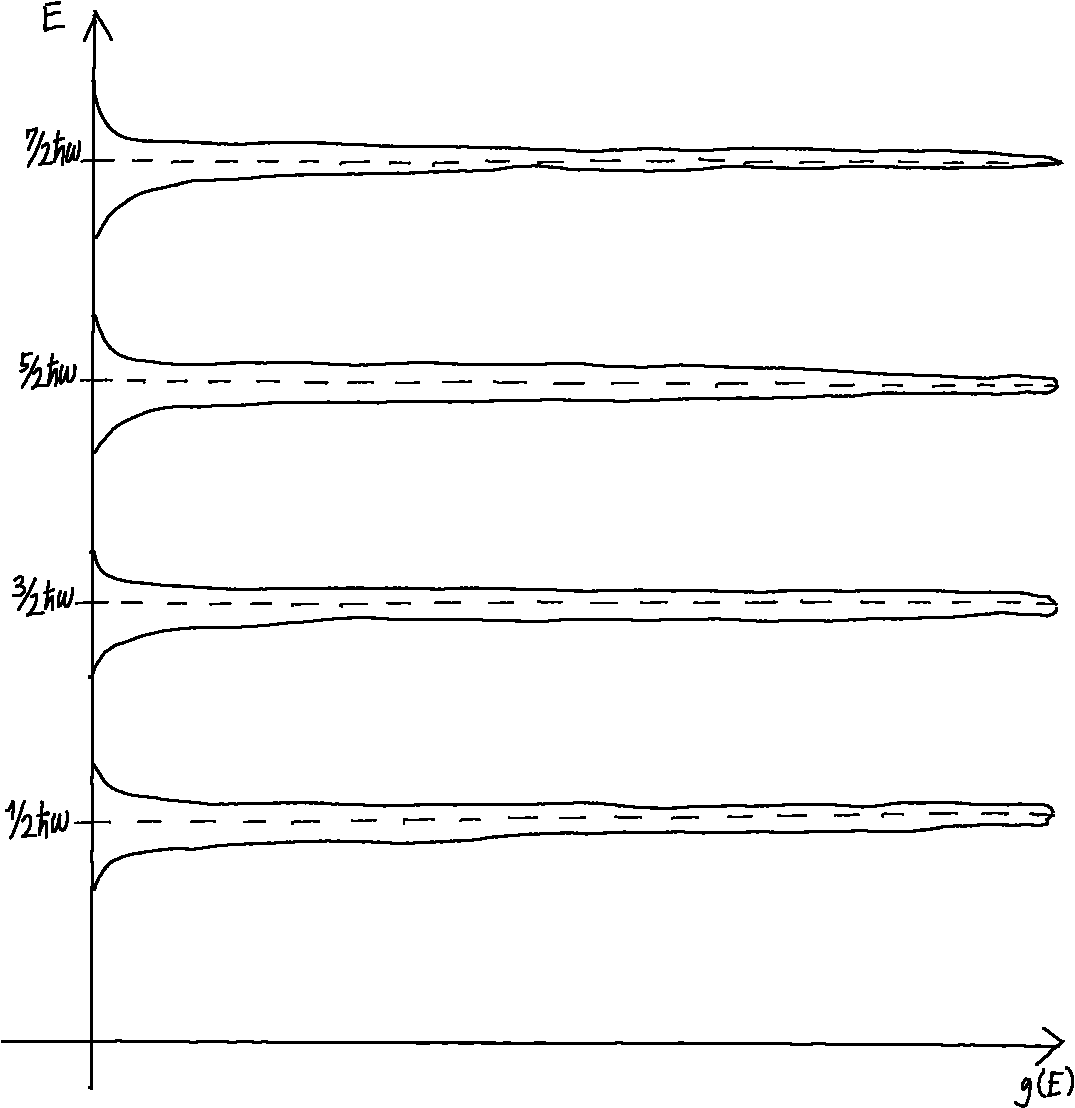
\includegraphics[width=.6\linewidth]{q3-dos}
	\end{figure}
	
	Resistivities:
	\begin{figure}[H]
		\centering
		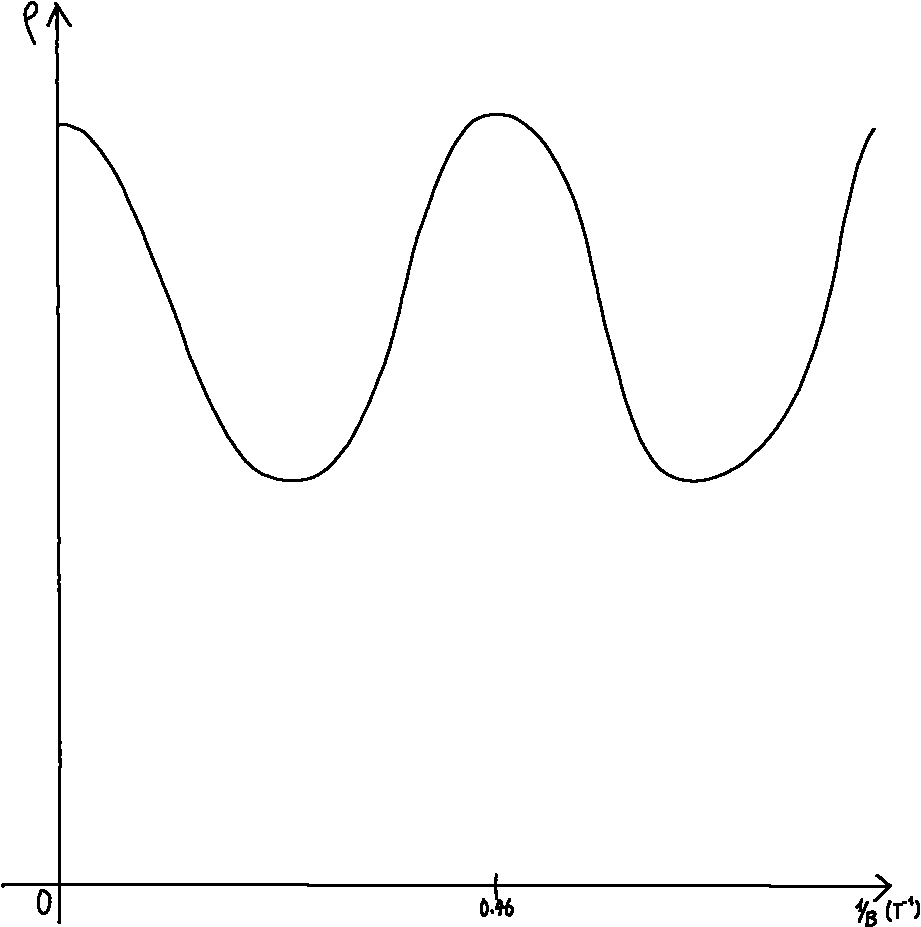
\includegraphics[width=.6\linewidth]{q3-rho}
	\end{figure}
	
	Hall resistance is quantised as it is dependent on the density of charge carrier, which is quantised due to the introduction of Landau levels:
	\begin{figure}[H]
		\centering
		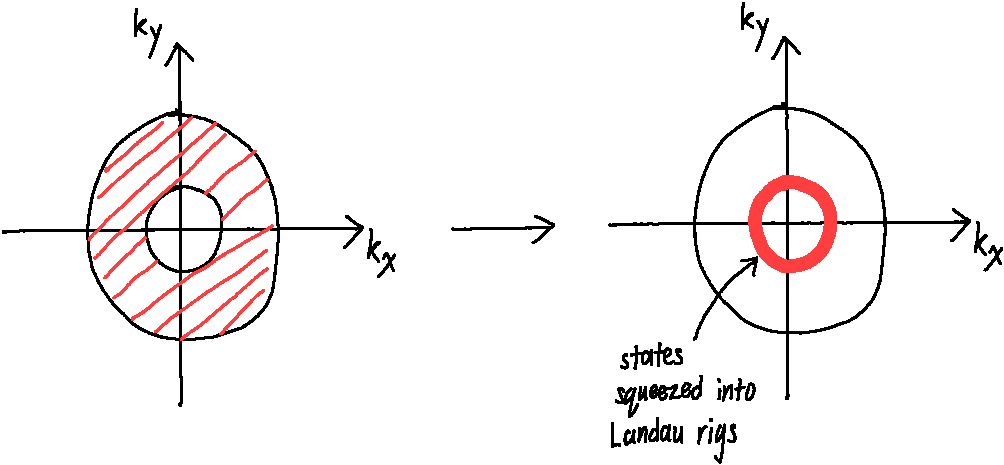
\includegraphics[width=.7\linewidth]{q3-landau-lvl}
	\end{figure}
	\textbf{\color{red}(WRONG)} The reason why this quantisation is precise is due to the density of states being partitioned precisely into the Landau levels as opposed to invoking correspondence principle which fails for small $l$.
	
	\part From Drude,
	\begin{align*}
		\deri{p}{t} &= f - \underbracket{\frac{p}{\tau}}_{\rightarrow 0 \mtext{as $\tau\rightarrow\infty$}} \\
		&= qE \\
		\Rightarrow m \deri{v}{t} &= qE \\
		\xRightarrow{J=nqv} \frac{m}{nq} \deri{J}{t} &= qE \\
		J &= \frac{nq^2}{m} Et
	\end{align*}
	for static voltage $V = El$ where $l$ is sample length.
	
	Conductance: $J = \sigma E$ $\Rightarrow$ since $n$ is quantised we have quantised $\sigma$ too.
	
	Unit of quantisation: ?
	
	We expect the quantisation here to be less precise due to the lack of correspondence principle???
\end{parts}